%KECReportFormat.tex
%%%%%%%%%%%%%%%%%%%%%%%%%%%%%%%%%%%%%%%%%%%%%%%%%%%%%%%%%%%%%%%%%%%%%%%%%%%
%DO NOT MAKE CHANGES IN THIS FILE

\documentclass[12pt, a4paper]{report}
\usepackage[left = 1.5in, right = 1in, top = 1in, bottom = 1in]{geometry}%for margin
\usepackage{amsfonts, amsmath, amssymb} %for mathematical equations
\usepackage{graphicx} %for images
\usepackage{times} %font Times New Roman Font
\usepackage{float} %required if you use H(strictly here) position for floats
\usepackage[skip = 8pt,tableposition=top, figureposition=bottom]{caption}%adjust spacing of captions and specify where captions are
\usepackage{hyperref} % for easy Navigation in document, also puts links in TOC, LOF, LOT...
\usepackage{setspace} %to change line spacing in some portion \singlespacing \onehalfspacing \doublespacing
\usepackage{acro} %for List of Abbrreviation and Symbol
\acsetup{first-style = short} % set to display only short form on the command \ac{}

%packages required for complex tables
\usepackage{bigstrut} 
\usepackage{multirow}

\renewcommand{\contentsname}{Table of Contents} %Change TOC Heading ... default is "Contents" 

\parindent 0pt	%removes the indent in paragraph
\setlength{\parskip}{18pt}	%for paragraph spacing
\renewcommand{\baselinestretch}{1.5}   %Line Spacing = 1.5 line-spaces

%to reduce spacing in sections
\usepackage{titlesec}
\titlespacing*{\section}{0pt}{0pt}{0pt} %left, top, bottom spacings
\titlespacing*{\subsection}{0pt}{0pt}{0pt}
\titlespacing*{\subsubsection}{0pt}{0pt}{0pt}
\titlespacing*{\paragraph}{0pt}{0pt}{0pt}
\titlespacing*{\subparagraph}{0pt}{0pt}{0pt}

%adjust fontsizes\ of sections
\titleformat*{\section}{\fontsize{14pt}{18pt}\bfseries}
\titleformat*{\subsection}{\fontsize{13pt}{18pt}\bfseries}
\titleformat*{\subsubsection}{\fontsize{12pt}{18pt}\bfseries}
\titleformat*{\paragraph}{\fontsize{12pt}{18pt}\bfseries}
\titleformat*{\subparagraph}{\fontsize{12pt}{18pt}\bfseries}

%to reduce separation between points in list
\usepackage{enumitem}
\setlist[enumerate]{nosep} % no separation between items in enumerate
\setlist[itemize]{nosep} % no separation between items in itemize
%use \vspace{-18pt} before list to reduce paragraph spacing between list and preceeding paragraph.

%Changes for Chapter Heading Spacing and formats for numbered chapters
\makeatletter
\def\@makechapterhead#1{%
  %\vspace*{50pt}%
  {  \MakeUppercase{\ifnum \c@secnumdepth >\m@ne
        \fontsize{16pt}{1}\bfseries \@chapapp \space \thechapter\vspace{5pt}\\
    \fi
    \interlinepenalty\@M
     \bfseries #1}\par\nobreak
    %\vskip 0pt
  }}
\makeatother

%%%%%%%%%%%%%%%%%%%%%%%%%%%%%%%%%%%%%%%%%%%%%%%%%%%%%%%%%%%
%to adjust Heading spacings and fonts For unnumbered chapters, TOC, LOF ...
\makeatletter
% Redefine the \chapter* header macro to remove vertical space
\def\@makeschapterhead#1{%
  %\vspace*{50\p@}% Remove the vertical space
  {\newpage \parindent \z@ \raggedright
    \normalfont
    \interlinepenalty\@M
    \center \fontsize{16pt}{1} \bfseries \MakeUppercase{#1}\par\nobreak
    %\vskip 18\p@ % adjust space after heading 18pt
  }}
\makeatother 
%%%%%%%%%%%%%%%%%%%%%%%%%%%%%%%%%%%%%%%%%%%%%%%%%%%%%%%%%%%

%%%%%%%%%%%%%%%%%%%%%%%%%%%%%%%%%%%%%%%%%%%%%%%%%%%%%%%%%%%%%%%%%%%%%%%%%%%
% newcommand for generating Cover Page
\newcommand{\KECcoverpage}
{
\begin{titlepage}
\begin{center}
\Large{\textbf{KANTIPUR ENGINEERING COLLEGE}}\\
\large{\textbf{(Affiliated to Tribhuvan University)}}\\
\large{\textbf{Dhapakhel, Lalitpur}}\\
\vfill	%vertically fill the space 
\begin{figure}[h] % h: put logo "here"
\begin{center}

\includegraphics[width=25mm, height = 25mm]{images/logo.png}
\end{center}
\end{figure}

\large{\textbf{[Subject Code: \subCode]}}\\ %Change This Line
\large{\textbf{A \MakeUppercase{\project} \MakeUppercase{\doc} ON}}\\ %Change This Line
\Large{\textbf{\MakeUppercase{\projectTitle}}}\\

\vfill	%vertically fill the space 
\large{\textbf{Submitted by:}}\\
\large{\textbf{\submittedBy}}\\
\vfill	%vertically fill the space 
\textbf{A \MakeUppercase{\project} SUBMITTED IN PARTIAL FULFILLMENT OF THE REQUIREMENT FOR THE DEGREE OF \MakeUppercase{\degree}}\\

\vfill	%vertically fill the space 
\large{\textbf{Submitted to:}}\\
\large{\textbf{\submittedTo}}\\
\vfill
\large{\textbf{\defMonth, \defYear}}
\pagebreak
\end{center}
\end{titlepage}
}
%%%%%%%%%%%%%%%%%%%%%%%%%%%%%%%%%%%%%%%%%%%%%%%%%%%%%%%%%%%%%%%%%%%%%%%
% newcommand for generating Cover Page
%Title Page
\newcommand{\KECtitlepage}
{
\begin{titlepage}
\begin{center}
\Large{\textbf{\MakeUppercase{\projectTitle}}}\\

\vfill	%vertically fill the space 

\large{\textbf{Submitted by:}}\\
\large{\textbf{\submittedBy}}\\


\ifhassupervisor % Displays Supervisor name only if \hassupervisortrue
	\vfill	%vertically fill the space 
	\large{\textbf{Supervised by:}}\\
	\large{\textbf{\supervisor}}\\
	\large{\textbf{\degSup}}\\
\fi

\vfill	%vertically fill the space 
\textbf{A \MakeUppercase{\project} SUBMITTED IN PARTIAL FULFILLMENT OF THE REQUIREMENT FOR THE DEGREE OF \MakeUppercase{\degree}}\\

\vfill	%vertically fill the space 
\large{\textbf{Submitted to:}}\\
\large{\textbf{\submittedTo}}\\
\large{\textbf{Kantipur Engineering College}}\\
\large{\textbf{Dhapakhel, Lalitpur}}\\

\vfill
\large{\textbf{\defMonth, \defYear}}
\thispagestyle{empty}\\ %to remove page number
\pagebreak
\end{center}
\end{titlepage}
}
%%%%%%%%%%%%%%%%%%%%%%%%%%%%%%%%%%%%%%%%%%%%%%%%%%%%%%%%%%%%%%%%%%%%%%
%command for copyright page
\newcommand{\KECcopyright}
{
\chapter*{Copyright}%Required only for Final Defense of Major Project
\addcontentsline{toc}{chapter}{Copyright}
The author has agreed that the library, Kantipur Engineering Collage, may make this report freely available for inspection. Moreover the author has agreed that permission for extensive copying of this report for scholarly purpose may be granted by the supervisor(s), who supervised the project work recorded herein or, in their absence, by the Head of the Department wherein this project was done. It is understood that due recognition will be given to the author of this report and to the \submittedTo, Kantipur Engineering College in any use of the material of this report. Copying or publication or other use of this report for financial gain without approval of the \submittedTo, Kantipur Engineering College and author’s written permission is prohibited.\par Request for permission to copy or to make any other use of the material in this report in whole or in part should be addressed to:

Head\\
\submittedTo\\
Kantipur Engineering College\\
Dhapakhel, Lalitpur\\
Nepal
}
%%%%%%%%%%%%%%%%%%%%%%%%%%%%%%%%%%%%%%%%%%%%%%%%%%%%%%%%%%%%%%%%%%%%%%
%command for Approval Letter
\newcommand{\KECapproval}
{
\chapter*{Kantipur Engineering College
\vskip -10pt}%Required only for Final Defense of Major Project
\begin{center}
\fontsize{12.8pt}{1} %size decreaced to adjust department name in single line
\textbf{
\MakeUppercase{\submittedTo}\\ %for department name
}
\vskip 10pt
\fontsize{16pt}{1}
\textbf{APPROVAL LETTER}
\end{center}
\vskip -16pt
\addcontentsline{toc}{chapter}{Approval Letter}%
The undersigned certify that they have read and recommended to the Institute of Engineering for acceptance, a project report entitled "\projectTitle " submitted by \\
\submittedBy \\
in partial fulfillment for the degree of \degree. \par
{\vspace{25pt}
..........................................\\
Supervisor\\
\supervisor \\
\degSup\\
\vspace{25pt}\\
..........................................\\
External Examiner\\
\external\\
\degExternal\\
\vspace{25pt}\\
..........................................\\
\hod\\
Head of Department\\
\submittedTo
\vspace{10pt}\\
Date: \defMonth\space\defDay ,\space \defYear
\singlespacing\par
} %single spacing for the texts inside {}
}

%command for list of abbreviations
\newcommand{\KECloa}
{
\chapter*{List of Abbreviations}
\addcontentsline{toc}{chapter}{List of Abbreviations}
\vskip -42pt % to reduce space due to invisivle acronym class name
{
\singlespacing
\printacronyms[include-classes=abbr, name= ]
}

}

%command for list of symbols
\newcommand{\KEClos}
{
\chapter*{List of Symbols}
\addcontentsline{toc}{chapter}{List of Symbols}
\vskip -42pt % to reduce space due to invisivle acronym class name{
{
\singlespacing
\printacronyms[include-classes=symbol, name= ]
}
}

%command to adjust toc, lof, lot spacing
\newcommand{\KECadjusttocspacings}
{
\parskip 0pt % to remove paragraph spacing in TOC, LOF ...
\renewcommand{\baselinestretch}{0.1} % to adjust line spacing in toc
\newcommand*{\noaddvspace}{\renewcommand*{\addvspace}[1]{}}
\addtocontents{lof}{\protect\noaddvspace} %remove extra vertical space in LOF
\addtocontents{lot}{\protect\noaddvspace} %remove extra vertical space in LOT
} %includes the file KecReportFormat.tex that include all necessary formattings
%%%%%%%%%%%%%%%%%%%%%%%%%%%%%%%%%%%%%%%%%%%%%%%%%%%%%%%%%%%%%%%%%%%%%%%%%%%
%Define Macros for Details of your Project
\newcommand{\project}{Major Project} %Specify "Major Project" or "Minor Project"
\newcommand{\projectTitle}{BRAIN TUMOR DETECTOR} %specify "Title" of Your Project
\newcommand{\doc}{Mid-Term Report} % specify the document you are preparing eg. "Proposal", "Mid-Term Report" or "Final Report" 
% Note that You have to sibmit "Final Report" for Pre-final defense as well.
\newcommand{\subCode}{CT755} %specify Subject of Your Project
\newcommand{\degree}{Bachelor in Computer Engineering} %specify your degree
\newcommand{\submittedBy}%Specify Names and Roll/Symbol Numbers of the Project Group Members
{
%Edit Member Names and Roll/Symbol No. and adjust width (\makebox[width]) if necessary 
\makebox[10cm]{Aliz Shrestha  \hfill[KAN076BCT009]}\\
\makebox[10cm]{Apurva Sharma Subedi \hfill[KAN076BCT016]}\\
\makebox[10cm]{Binit Shakya    \hfill[KAN076BCT022]}\\
\makebox[10cm]{Kashyap Ghimire     \hfill[KAN076BCT037]}
%\makebox[9cm]{Member Name \hfill [Roll/Symbol No.]}\\
} % Note that You must write your "Symbol Numbers"(Exam Roll Numbers) for Final Defenses

\newcommand{\submittedTo}{Department of Computer and Electronics Engineering} %specify your department
\newcommand{\hod}{Er. Rabindra Khati} %specify Head ot the department
\newcommand{\defYear}{2023} %Defense Year
\newcommand{\defMonth}{December} %Defense Month- January, February, ...
\newcommand{\defDay}{25} %specify Defense Day- 1, 2, ...

\newif\ifhassupervisor
\hassupervisortrue % to display supervisor name use command- \hassupervisortrueb
\newcommand{\supervisor}{Er. Binod Wosti} % Specify Name of Supervisor for Major Project (write "none" if no Supervisor is assigned)
\newcommand{\degSup}{Computer Engineer\\CIAA} %Specify Designation of Supervisor for Major Project, use multiple lines (\\) if necessary
\newcommand{\external}{External's Name} %Specify Name of External for Major Project (Required for Black Book)
\newcommand{\degExternal}{External's Designation\\Second Line of Designation (if required)} %Specify Name of External for Major Project (Required for Black Book) , use multiple lines (\\) if necessary
%%%%%%%%%%%%%%%%%%%%%%%%%%%%%%%%%%%%%%%%%%%%%%%%%%%%%%%%%%%%%%%%%%%%%%%%%%%

%%%%%%%%%%%%%%%%%%%%%%%%%%%%%%%%%%%%%%%%%%%%%%%%%%%%%%%%%%%%%%%%%%%%%%%%%%%

%%%%%%%%%%%%%%%%%%%%%%%%%%%%%%%%%%%%%%%%%%%%%%%%%%%%%%%%%%%%%%%%%%%%%%%%%%%%%%%%%%%%%%%%%%%%%%%%%%%%

%%%%%%%%%%%%%%%%%%%%%%%%%%%%%%%%%%%%%%%%%%%%%%%%%%%%%%%%%%%%%%%%%%%%%%%%%%
%The Document
\setcounter{tocdepth}{3}
\setcounter{secnumdepth}{3}
\begin{document}

\KECcoverpage  
\KECtitlepage
\pagenumbering{roman} % starts pagenumberins in Roman numerals i, ii, ...

%Copyright Page is required for FINAL REPORT only. Comment this section for other Reports.
%\KECcopyright % defined in KECReportFormat.tex

%Approval Page is required for FINAL(Black Book Binded) REPORT of MAJOR PROJECT only. Comment this section for other Reports. 
%\KECapproval % defined in KECReportFormat.tex

%\chapter*{Abstract} % The summary of your report
%\addcontentsline{toc}{chapter}{Abstract}%to include this chapter in TOC 
%In the current world, many people are suffering from various medical conditions, due to which the number of patients approaching hospitals to perform their regular check-ups have increased drastically. For regular routine check-ups, most of these patients will sign up to perform body check-ups in which Magnetic Resonance Imaging(MRI) scanning is widely used in order to observe the condition and state of the internal organs. As a result of these cases, the number of MRI scans that are to be viewed and reviewed by the doctors will be high. Due to which in some cases the doctors may get tired and their performance and efficiency may reduce. As a result of which, there may be some inconsistency in the diagnosis and treatment process. In the medical field, these types of inconsistencies may lead to fatal cases and improper diagnosis. So, to solve this issue by using highly accurate deep learning concepts and algorithms is necessary as the efficiency, sustainability and computation of computers far exceeds human capabilities. So, in order to provide diagnostic accuracy and provide early detection of high risk cases such as brain tumors, these kinds of deep learning practices can be used. In this project, a Convolution Neural Network (CNN) based model known as AlexNet will be used in order to extract features and another CNN based model Support Vector Machine(SVM) will be used to detect brain tumors, for which the dataset available on Kaggle  will be used.
%\par
%\textbf{\textit{Keywords$-$}} \emph{Magnetic Resonance Imaging, Tumor, Convolution Neural Network, AlexNet, Kaggle
%}

%\chapter*{Acknowledgment}
%\addcontentsline{toc}{chapter}{Acknowledgment}%to include this chapter in TOC
%We would like to express sincere gratitude to Department head Er. Rabindra Khati, Project Co-ordinator Er. Bishal Thapa and all the faculty members of Kantipur Engineering College for the continuous support during this project for their patience, motivation,enthusiasm, and immense knowledge. Their guidance helped us in all time of research, development and implementation of this project.   \par
%Finally we would like to thank our family and friends for all the support and encouragement.\par
%to display members name under Acknowledgement
%\begin{flushright}
%\vskip -20pt
%\setstretch{1.2}
%\submittedBy

%\end{flushright}

%to adjust spacings for TOC, LOF, LOT
{
%%%%%%%%%%%%%%%%%%%%%%%%%%%%%%%%%%%%%%%%%%%%%%%%%%%%%%%%%%%%%%%%%%%%%%%%%%%
%TOC, LOF and LOT
\KECadjusttocspacings % defined in KECReportFormat.tex to adjust spacings
\makeatletter
% to add vskip of 18 point which is reduced when parskip is set to 0 in \LECadjustspacings
\def\@makeschapterhead#1{%
  %\vspace*{50\p@}% Remove the vertical space
  {\newpage \parindent \z@ \raggedright
    \normalfont
    \interlinepenalty\@M
    \center \fontsize{16pt}{1} \bfseries \MakeUppercase{#1}\par\nobreak
   % \vskip 18\p@ % adjust space after heading 18pt
  }}
\makeatother 

\tableofcontents % prints table of contents
\listoffigures % prints list of figures
\addcontentsline{toc}{chapter}{List of Figures}
\listoftables % prints list of table
\addcontentsline{toc}{chapter}{List of Tables}
}
%%%%%%%%%%%%%%%%%%%%%%%%%%%%%%%%%%%%%%%%%%%%%%%%%%%%%%%%%%%%%%%%%%%%%%%%%%%
\chapter*{List of Abbreviations}
\makebox[3cm]{CNN:}   Convolution Neural Network\\
\makebox[3cm]{SVM:}   Support Vector Machine\\
\makebox[3cm]{YOLO:}  You Only Look Once\\
\makebox[3cm]{MRI:}   Magnetic Resonance Imaging\\
%2D:    2 Dimensional\\
%3D:    3 Dimensional\\
%CNN:   Convolution Neural Network\\
%DICOM: Digital Imaging and Communications in Medicine\\
%MRI:   Magnetic Resonance Imaging\\
%PC:    Personal Computer



\addcontentsline{toc}{chapter}{List of Abbreviations}
%comment this chapter if you don't have List of Abbreviations
%\KECloa % defined in KECReportFormat

%comment this chapter if you don't have List of Symbols
%\KEClos % defined in KECReportFormat

\newpage
\pagenumbering{arabic} % starts pagenumbering in arabic numerals

\chapter{Introduction}
\vspace{-18pt}
\section{Background}\label{sec:bkgrnd}%label your section if you require to refer them somewhere else in your document.
\vspace{-18pt}
In the field of medical imaging, Magnetic Resonance Imaging (MRI) has emerged as a powerful tool for diagnosing and monitoring various medical conditions. MRI scans provide detailed images of internal organs, tissues, and structures within the body, enabling healthcare professionals to detect abnormalities and plan appropriate treatment strategies. However, the interpretation of MRI scans can be complex and can be in large numbers, requiring expertise and experience to accurately analyze the voluminous data generated by these scans\cite{Mirchandani}.
\par
 The detection of brain tumors plays a crucial role in early diagnosis and treatment planning. In recent years, deep learning algorithms have shown remarkable performance in medical image analysis\cite{ZainEldin2023}. One such algorithm is AlexNet, a convolutional neural network (CNN) that has proven effective in various computer vision tasks. The objective of this project is to leverage the power of AlexNet for brain tumor detection\cite{Mirchandani}. The proposed method involves training the AlexNet architecture on a large dataset of brain MRI images, consisting of both tumor and non-tumor cases. The network learns to extract distinctive features from the images through multiple convolutional and pooling layers. Once the features are obtained from the AlexNet model, they are fed into an SVM classifier. SVM is a popular machine learning algorithm known for its effectiveness in binary classification tasks\cite{Sejuti2021}. The SVM learns to differentiate between tumor and non-tumor cases based on the extracted features from the AlexNet model.The final classification layer is modified to output a binary prediction indicating the presence or absence of a brain tumor where ‘0’ will show that the test image is tumor free and ‘1’ will show that the test image has a tumor.
 \par
 The introduction of “Brain Tumor Detector” provides the feature of detection of various kinds of brain tumor using deep learning techniques in order to provide accurate detection and representation of the portion of the brain that has the tumor cell present in it.

\section{Problem Statement}
\vspace{-18pt}
The development of a computer system capable of automatically and accurately detecting brain tumors in MRI scans is the focus of this project. The conventional manual analysis of medical images for brain tumor detection is time-consuming and prone to human errors. To overcome these limitations, the project aims to leverage the capabilities of the AlexNet convolutional neural network (CNN) algorithm.
\par
By training the AlexNet model on a large dataset of labeled brain MRI images, the model can learn to extract essential features for distinguishing between tumor and non-tumor cases. The complexity of MRI images and the need to minimize false alarms pose challenges that must be addressed.

\section{Objectives}
\vspace{-18pt}
The main objectives of this application are mentioned below:
\vspace{-18pt}
\begin{enumerate}[label=\roman*.]
\item To accurately detect tumors using deep learning.

\end{enumerate}
\section{Project Features}
\vspace{-18pt}
The application is targeted toward the general population. So the features of this application can be listed below:
\vspace{-18pt}
\begin{enumerate}[label=\roman*.]
\item Detect tumor based on input MRI scanned images
\item Provides the interface for loading the MRI images and check the results
\item Use deep learning techniques for training the data sets for higher accuracy.
\end{enumerate}
\section{Application Scope}
\vspace{-18pt}
Brain Tumor Detector has a diverse range of applications in medical imaging, diagnosis, treatment planning, patient education, and research. These advanced tools enhance the interpretation of MRI scans by providing accurate prediction, enabling accurate and early diagnoses and improved surgical planning\cite{Saeedi2023}. They also contribute to medical research and education by facilitating detailed anatomical study of possible cases of brain tumors.
\section{System Requirement}
\vspace{-18pt}
\subsection{Development Requirements}
\vspace{-18pt}
\subsubsection{Software Requirements}
\vspace{-10pt}
\begin{itemize}
\item Windows/Linux/Mac
\item Python IDE
\item QT Designer
\end{itemize}
\subsubsection{Hardware Requirements}
\vspace{-10pt}
\begin{itemize}
\item PC with 16 GB RAM
\item Graphics with 4 GB dedicated memory
\end{itemize}
\subsection{Deployment Requirements}
\vspace{-18pt}
\subsubsection{Software Requirements}
\vspace{-10pt}
\begin{itemize}
\item Windows 10


\end{itemize}
\vspace{-10pt}
\subsubsection{Hardware Requirements}
\vspace{-10pt}
\begin{itemize}
\item CPU with 1.5 GHz clock speed
\item 8 GB RAM
\end{itemize}
\label{tblSampleTable}
%\end{table}
\section{Project Feasibility}
\vspace{-18pt}
\subsection{Technical Feasibility}
\vspace{-18pt}
Technically, the system is feasible enough for most users, but a basic familiarity with the applications is expected from the users.
\vspace{-18pt}
\subsection{Operational Feasibility}
\vspace{-18pt}
The user will not need any formal knowledge about programming so our project is operationally feasible.
\vspace{-18pt}
\subsection{Economic Feasibility}
\vspace{-18pt}
The purpose of the economic feasibility assessment is to determine the positive economic benefits to the user that the proposed system will provide. Most of the software used for the development is free. Thus, the project is economically feasible.
\vspace{-18pt}
\subsection{Schedule Feasibility}
\begin{figure}[!h] % tbh means top, bottom or here (priority: left to right)
\begin{center}
	%
\includegraphics[width = in]{images/logo.png}
	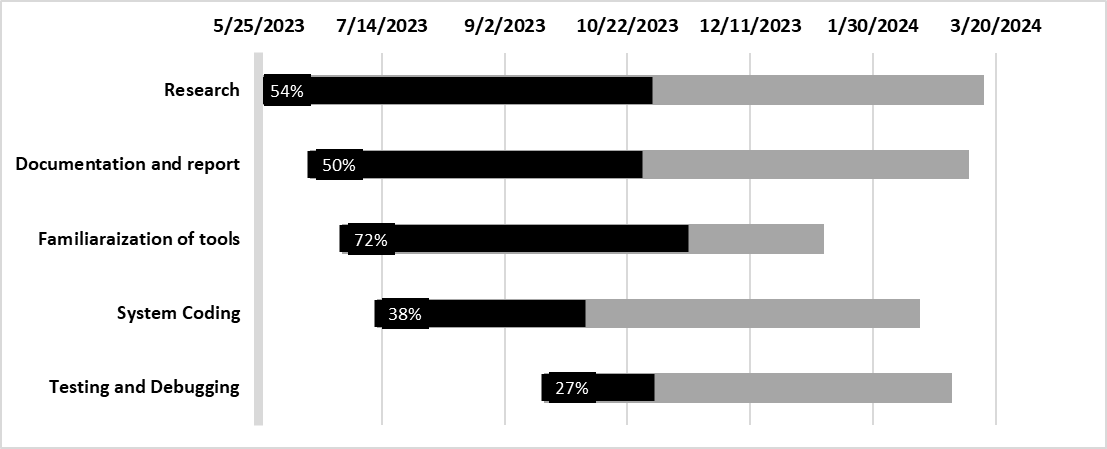
\includegraphics[width=6in]{images/gc2.png} 
	\caption{Gantt Chart} %figure name
	\label{fig 1 GanttChart} % for referencing
\end{center}
\end{figure}
\chapter{Literature Review}
\vspace{-18pt}
\section{Related Projects}
\vspace{-18pt}
\subsection{
Brain Tumor Segmentation (BraTS) Software:}
\vspace{-18pt}
BraTS is a widely used software for brain tumor segmentation, which involves identifying and delineating tumor regions in MRI scans. It utilizes CNN-based algorithms to analyze the image data and generate precise tumor segmentation maps.
 \vspace{-10pt}
\subsection{MIPAV:}
\vspace{-18pt}
Medical Image Processing, Analysis, and Visualization (MIPAV) is a software package developed by the National Institutes of Health (NIH). It offers a range of tools for tumor detection, including automated segmentation algorithms, image registration, and quantitative analysis.
\vspace{-10pt}
\subsection{ImageJ:}
\vspace{-18pt}
ImageJ is an open-source image processing software widely used in medical research and clinical practice. It provides a range of plugins and tools for tumor detection and analysis, including segmentation algorithms and quantitative measurements.   
\vspace{-10pt}

\section{Related Research}
\vspace{-18pt}
A CNN-SVM based method is proposed to classify brain tumor with higher accuracy. Firstly, a convolutional neural network having 19 layers is constructed using three convolutional 2D layers, three max-pooling layers, two fully-connected layers, three batch normalization layers with activation functions reLu. Secondly softmax is used as a classifier and implemented over a dataset containing 3064 images on three class of tumor images (glioma tumors,meningioma tumors, and pituitary tumors). After that, another classifier named support vector machine is used to improve the accuracy of the CNN model using the features extracted from the model. The final accuracy of this proposed CNN-SVM based method is found 97.1\% \cite{Sejuti2021}.
\newpage
 
\par
For the next research work we looked did a study whose aim was to utilize three well-known CNN-based algorithms, AlexNet, Faster R-CNN, and YOLOv4 to perform multiclass classification of brain MRI scans of Alzheimer Disease patients.
 
  \begin{center}
	\begin{table}[H]
	\centering
	\begin{tabular}{lllll}
	\cline{1-4}
	\multicolumn{1}{|l|}{Classifiers} & \multicolumn{1}{l|}{AlexNet} & \multicolumn{1}{l|}{Faster R-CNN} & \multicolumn{1}{l|}{YOLOv4} &  \\ \cline{1-4}
\multicolumn{1}{|l|}{Loss}        & \multicolumn{1}{l|}{0.02}    & \multicolumn{1}{l|}{0.3}          & \multicolumn{1}{l|}{0.7}    &  \\ \cline{1-4}
\multicolumn{1}{|l|}{Accuracy}    & \multicolumn{1}{l|}{99\%}    & \multicolumn{1}{l|}{41\%}         & \multicolumn{1}{l|}{86\%}   &  \\ \cline{1-4}
                                  &                              &                                   &                             & 
\cite{Mirchandani}
\end{tabular}
\caption{Comparision table Of CNN architecture}
\label{Comparision table Of CNN architecture}
\end{table}
\end{center}
\chapter{Methodology}
\vspace{-18pt}
  \section{Working Mechanism}
  \vspace{-18pt}
  \subsection{Block Diagram}
  \vspace{-18pt}
A block diagram is a drawing illustration of a system whose parts are illustrated by blocks. These blocks are joined by lines to display the relationship between the blocks. Block diagrams are used to visualize the functionality of a system.
\begin{figure}[tbh] % tbh means top, bottom or here (priority: left to right)
\begin{center}
	%
\includegraphics[width = 3in]{images/logo.png}
	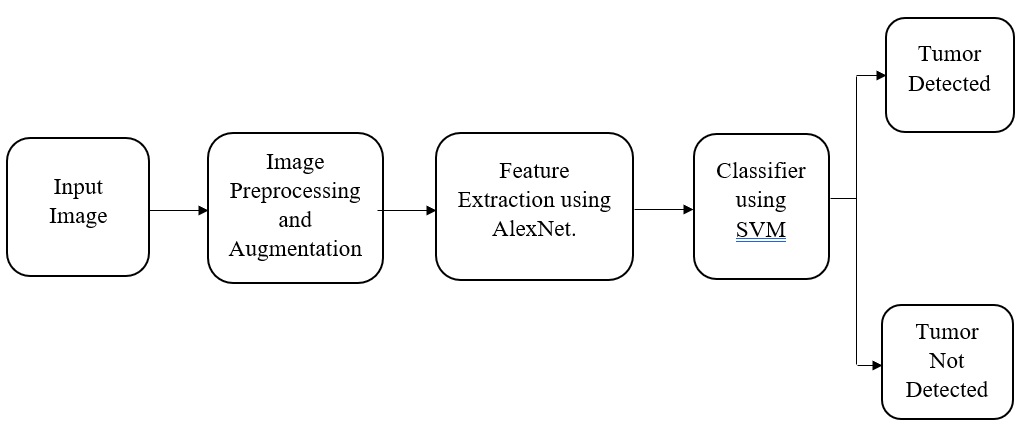
\includegraphics[width=3in]{images/systemBlock.png} 
	\caption{ System Block Diagram} %figure name
	\label{System Block Diagram} % for referencing
	
\end{center}
\end{figure}
\par
Input images of MRI scan are provided to the system. Then the data is preprocessed to make it easy for classification purposes. Then the data is augmented after which AlexNet architecture of CNN model extracts the features of the provided image.The output from AlexNet is then fed to the SVM model that has learned from the training dataset, it classifies the images as tumor detected or not.
\subsection{Input data}
\vspace{-18pt}
Firstly, the dataset that is used to train the model is taken and classified into testing, validation and training datasets. The testing dataset is used in order to train the deep learning algorithm, the validation dataset is then used to validate the model and the test dataset is used to test the model performance metrics such as accuracy, sensitivity and specificity. The training data we will be using has been taken from kaggle and has already been seperated into two category in relation to the presence of tumor.There are 155 jpg image that have tumor and 98 jpg image that are tumor free.
\subsection{ Data preprocessing}
\vspace{-18pt}
After the dataset has been gathered and classified into training and testing sets, they need to be preprocessed. Data preprocessing is an essential step in CNN image classification, aimed at improving the quality and efficiency of the classification process. It involves several techniques to prepare the input data before feeding it into the network.
\par
 %

\subsection{Data augmentation}
\vspace{-18pt}
Data augmentation is a technique used in deep learning for image classification to create more training examples by making changes to the original images. These changes help improve the model's ability to understand different variations of the same object. The common ways of doing data augmentation are:
\begin{description}
\item[1. Flipping] \hfill \\
 The images are flipped horizontally or vertically to help the model recognize objects from different angles.
\item[2. Rotating] \hfill \\
 The images are rotated by different angles to help the model handle objects that are not upright.
 \item[3. Cropping] \hfill \\
 Parts of the images are randomly cut out to teach the model to focus on important parts of an object.
 \item[4. Scaling] \hfill \\
The size of the images is changed to help the model recognize objects at different scales.
 \item[5. Adjusting Colors] \hfill \\
 The colors of the images are changed slightly to help the model handle variations in lighting and color.
 Random noise is added to the images to make the model more robust to imperfections in real-world images.
\end{description}
\par 

By using these techniques, we can create more diverse training data, which helps the model learn better and perform well on new and unseen images.




\subsection{Feature Extraction}
\vspace{-18pt}
For feature extraction of the datasets we will be using AlexNet model of CNN. This model of CNN is chosen because of its better performance compared to similar models such as YOLOv4 and R-CNN \cite{Mirchandani}.

\begin{description}
\item[AlexNet] \hfill \\
AlexNet is a deep convolutional neural network (CNN) that was introduced in 2012 by Alex Krizhevsky, Ilya Sutskever, and Geoffrey Hinton. It gained significant attention and achieved breakthrough performance in the ImageNet Large Scale Visual Recognition Challenge (ILSVRC) competition.
\begin{figure}[tbh] % tbh means top, bottom or here (priority: left to right)
\begin{center}
	%
\includegraphics[width = 3in]{images/logo.png}
	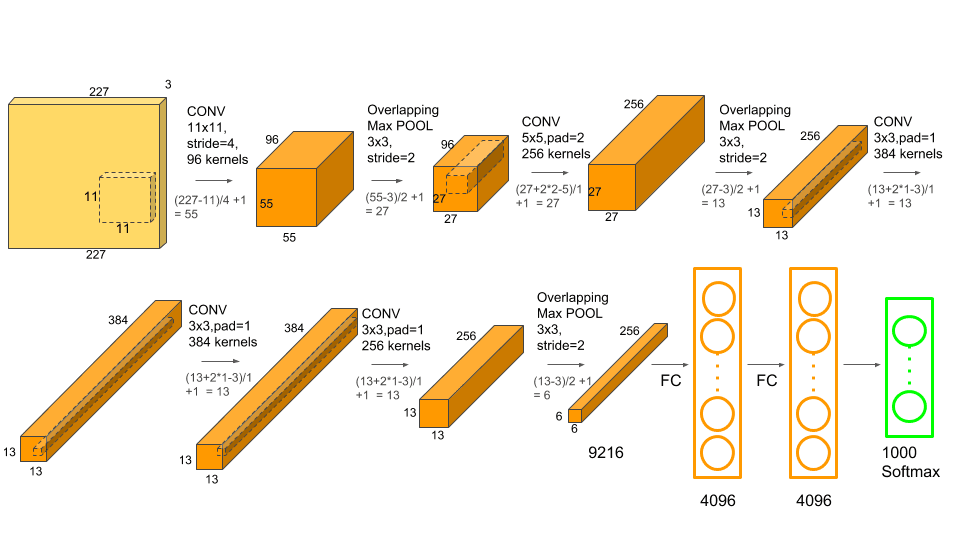
\includegraphics[width=4in]{images/Alexnet2.png}
	\caption[Architecture of Alexnet]{\centering Architecture of Alexnet \\Source: \textit{https://towardsdatascience.com/transfer-learning-using-pre-trained-alexnet-model-and-fashion-mnist-43898c2966fb}} %figure name
	
	\label{Architecture of Alexnet } % for referencing
	
\end{center}
\end{figure}
\end{description}
Here's a step-by-step overview of how AlexNet works up to the feature extraction stage:
\begin{description}
\item[1. Input Image:]
The network takes an input image with dimensions typically set to 224x224 pixels.
\item[2. Convolutional Layers:]
The input image passes through a series of convolutional layers. These layers consist of learnable filters that scan the input image, extract local features, and produce feature maps. AlexNet has a total of five convolutional layers.
When we apply a filter of size [f*f] with stride 's' on an padded image of size [n1*n2] we obtain an output of size:\\

\begin{equation}
\Large
\left\lfloor\frac{n_{1}-2p-f}{s}+1\right\rfloor*\left\lfloor\frac{n_{2}-2p-f}{s}+1\right\rfloor
\label{1}
\end{equation}

\item[3. ReLU Activation:]
After each convolutional layer, a rectified linear unit (ReLU) activation function is applied element-wise to introduce non-linearity. ReLU sets all negative values in the feature maps to zero while leaving the positive values unchanged.
\item[4. Pooling Layers:]
The feature maps are then passed through pooling layers to downsample the spatial dimensions. AlexNet uses max pooling, where the maximum value within each pooling window is retained, reducing the spatial size while preserving important features.
\item[5. Local Response Normalization (LRN):]
LRN is applied after some of the pooling layers in AlexNet. It normalizes the responses across different feature maps to enhance the contrast between local responses. This helps with generalization and provides a form of competition between features.
\end{description}
\par 
After several convolutional and pooling layers, the output is flattened into a one-dimensional vector that is fed into the SVM model for classification
\subsection{Classification}
\vspace{-18pt}
After we have extracted the feature from the given images we then feed the flattened one-dimensional vector into the SVM so that it can be classified.
\newpage
\begin{description}
\item[SVM] \hfill \\
SVM operates in the context of a classification problem, where the goal is to assign an input sample to one of the predefined classes
\begin{figure}[tbh] % tbh means top, bottom or here (priority: left to right)
\begin{center}
	%
\includegraphics[width = 3in]{images/logo.png}
	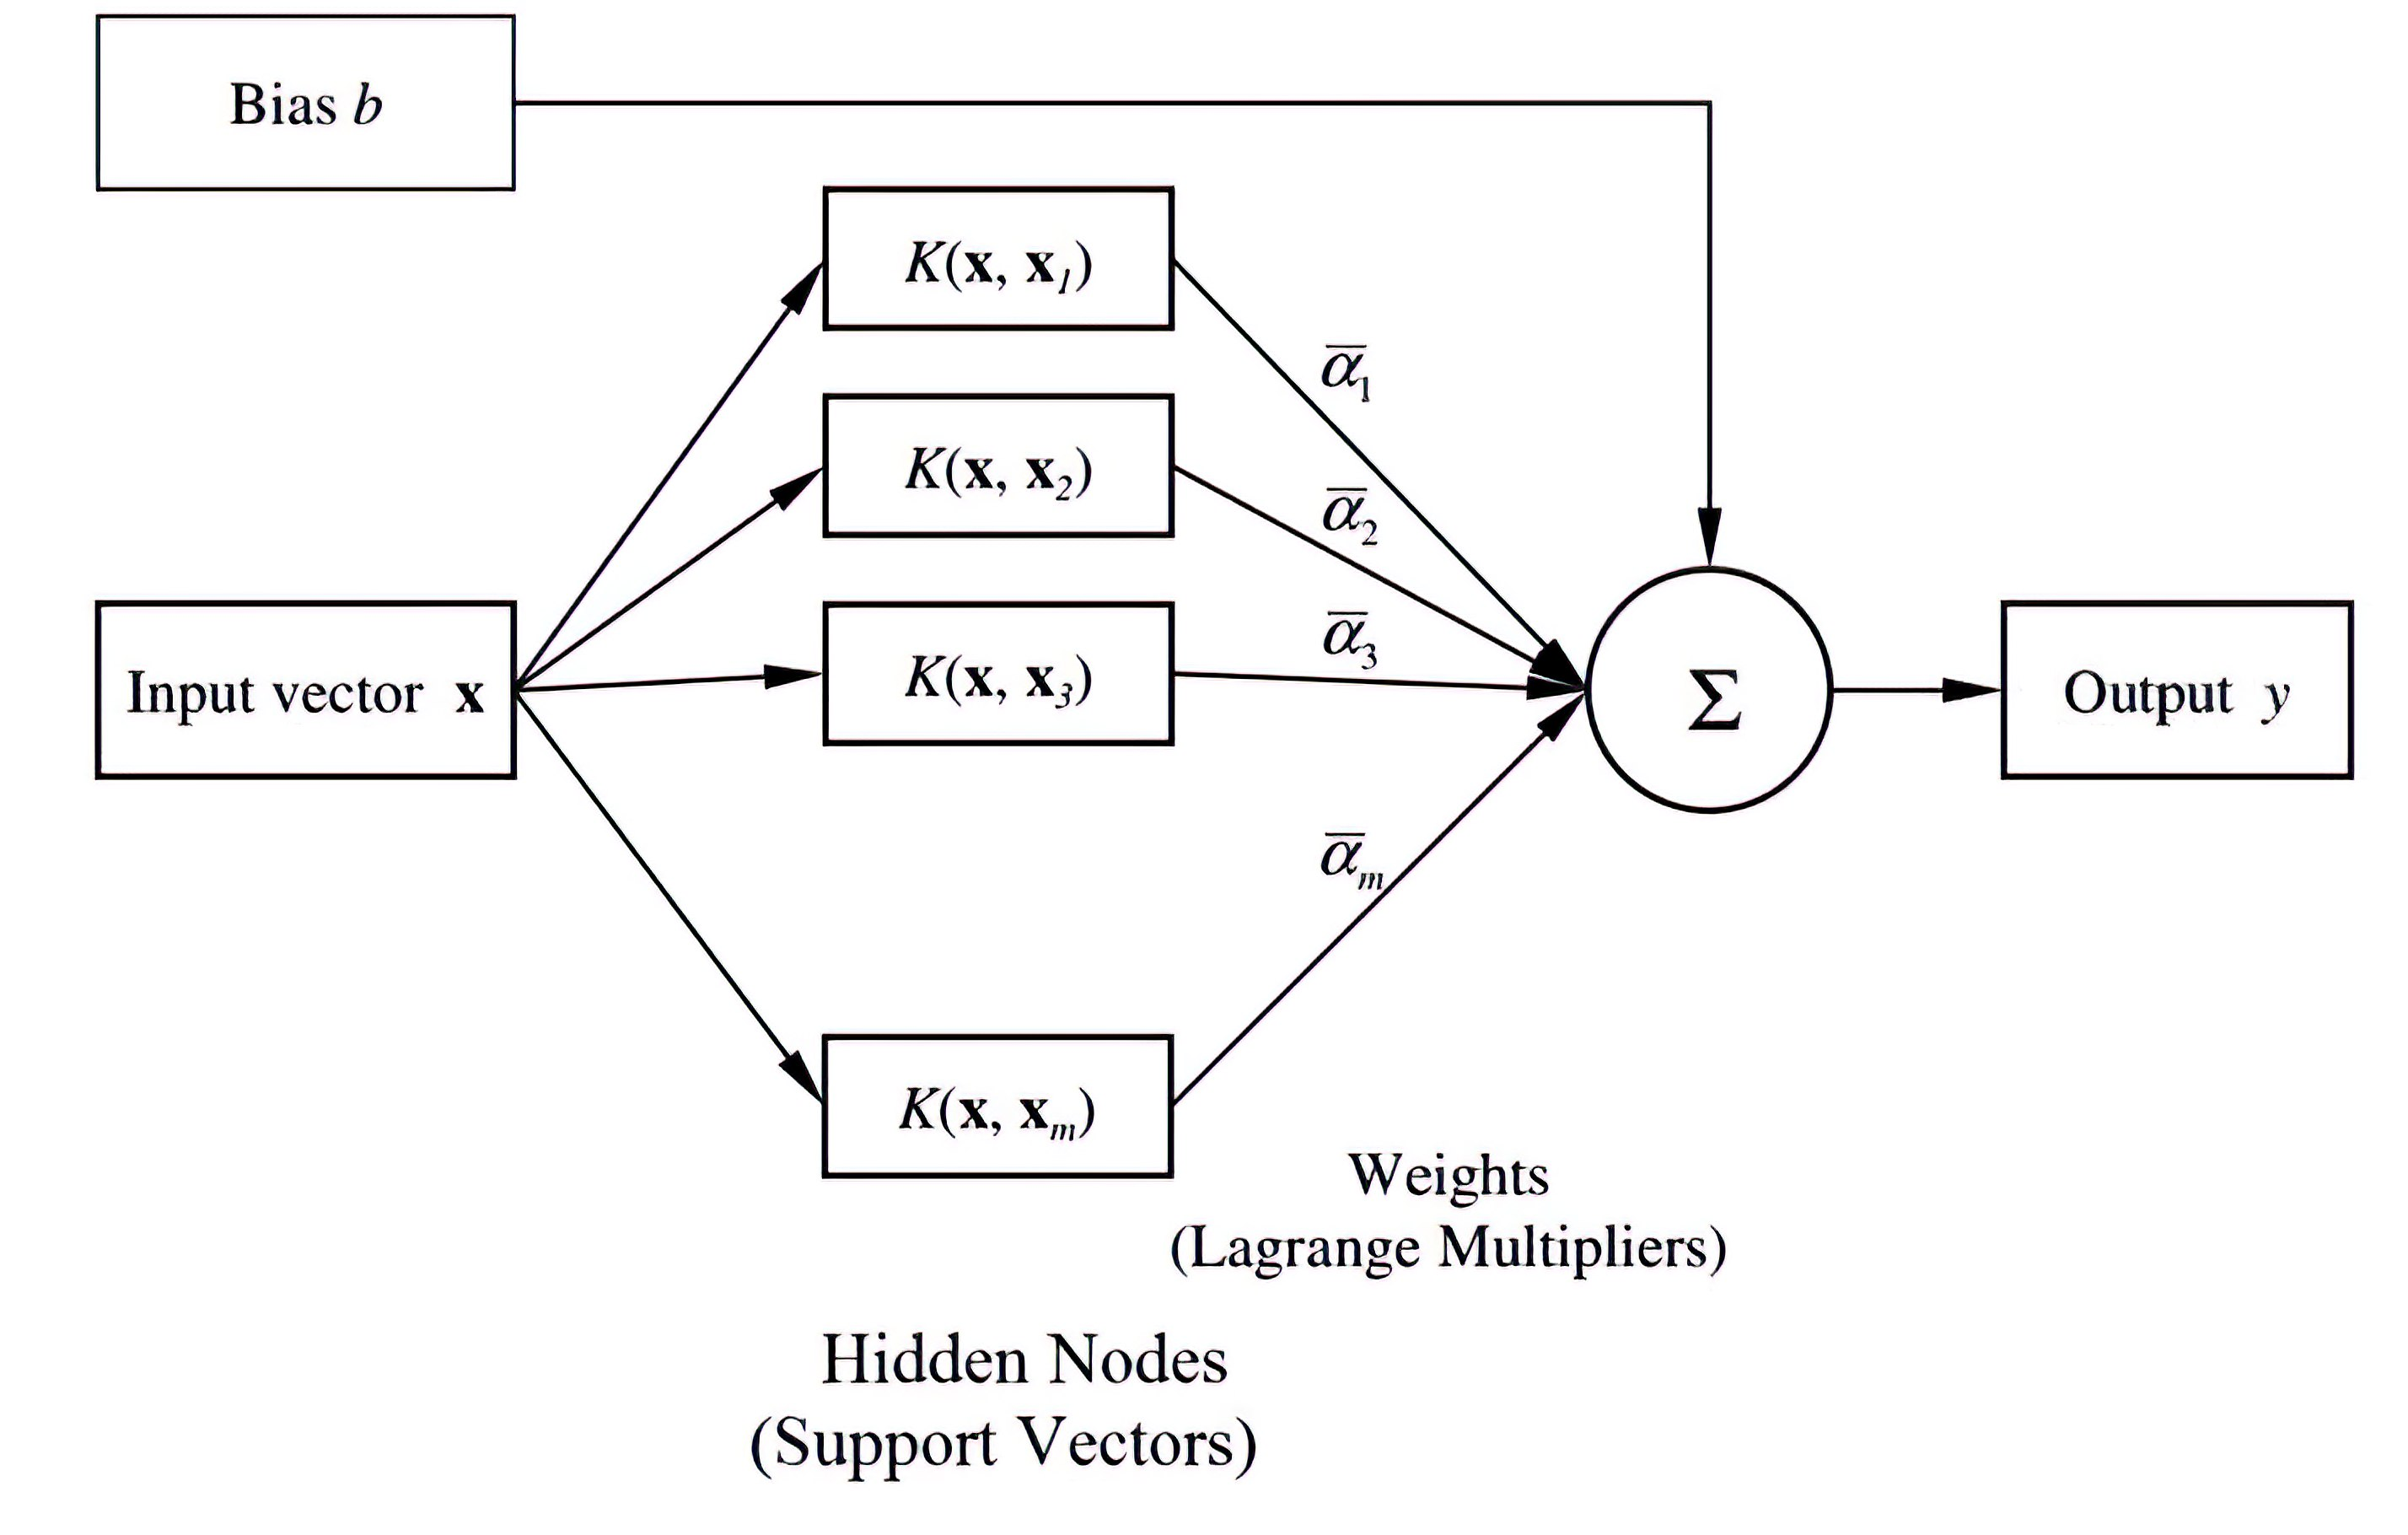
\includegraphics[width=5in]{images/svm.jpg} 
	\caption[Schematic diagram of SVM]{ \centering Schematic diagram of SVM
	\\Source:\textit{https://www.researchgate.net/figure/Schematic-diagram-of-SVM-architecture_fig1_317701295} } %figure name
	
	\label{Schematic diagram of SVM  } % for referencing
	
\end{center}
\end{figure}
\newpage
\begin{description}
\item[1. Feature Vector:]The feature vector obtained from the fully connected layers serves as the input to the SVM classifier. This feature vector represents the extracted features from the input image.
\item[2. Training Data:]A labeled training dataset is required to train the SVM. The dataset consists of feature vectors from various samples along with their corresponding class labels.
\item[3. Feature Scaling: ]Before training the SVM, it's common practice to perform feature scaling on the feature vectors. This ensures that all features have similar scales and prevents any particular feature from dominating the learning process.
\item[4. Support Vectors:]During the training phase, SVM identifies a subset of training samples called support vectors. These support vectors are the samples that lie closest to the decision boundaries between different classes.
\item[5. Hyperplane:]SVM finds an optimal hyperplane in the high-dimensional feature space that best separates the different classes. This hyperplane maximizes the margin or distance between the closest support vectors from each class.
\item[6. Kernel Trick: :]SVM can employ a kernel function to transform the feature vectors into a higher-dimensional space, enabling the classification of non-linearly separable data. Common kernel functions include linear, polynomial, radial basis function (RBF), and sigmoid.
\item[7. Decision Function:]After training, SVM constructs a decision function based on the support vectors and their associated weights. This function takes a new feature vector as input and assigns it to one of the classes based on its position relative to the learned decision boundary.
\item[8. Prediction:]To predict the class label of a new sample, the SVM classifier applies the decision function to its feature vector. The output of the decision function determines the class assignment.
\end{description}
\end{description} 
\newpage
\section{System Diagram}
\vspace{-18pt}
\subsection{Use case diagram}
\vspace{-18pt}
A use case diagram is a way to summarize the details of a system and the users within that system. It is generally shown as a graphic depiction of interactions among different elements in a system. Use Case Diagrams will specify the events in a system and how those events flow. However, Use Case Diagram does not describe how those events are implemented.
\begin{figure}[h]
\begin{center}
	%
\includegraphics[width = 3in]{images/logo.png}
	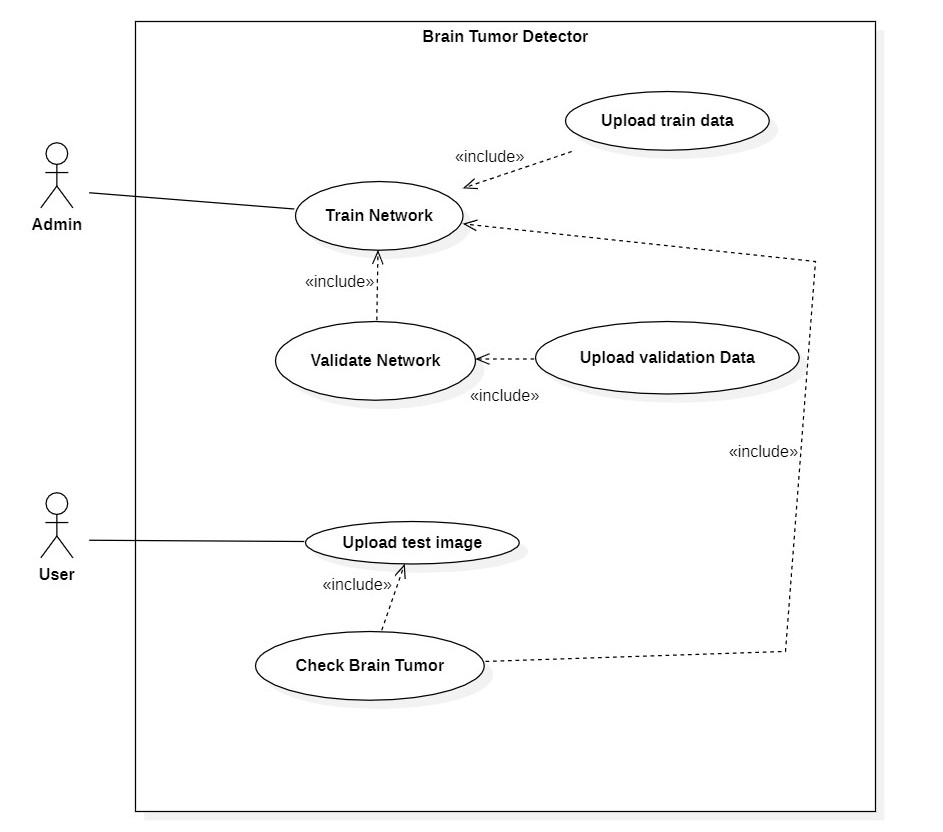
\includegraphics[width=5in]{images/ucd.jpg} 
	\caption{Use Case Diagram of Brain Tumor Detector} %figure name
	\label{Use Case Diagram of Brain Tumor Detector} % for referencing
\end{center}
\end{figure}

\subsection{Software Development Model}
\vspace{-18pt}
One of the software development life cycle models that is easy to apply is the incremental approach. In some cases, the original or fundamental software requirements are well recognized, but the project's actual scope or complete set of features is not. Additionally, the software development company might opt not to provide the entire functionality of the program at once. Instead, they want to distribute it through routine updates, or if the client demands some functionality upgrades while the project is still being developed Then in these situations, the incremental model is applied.
 \begin{figure}[tbh] % tbh means top, bottom or here (priority: left to right)
\begin{center}
	%
\includegraphics[width = 3in]{images/logo.png}
	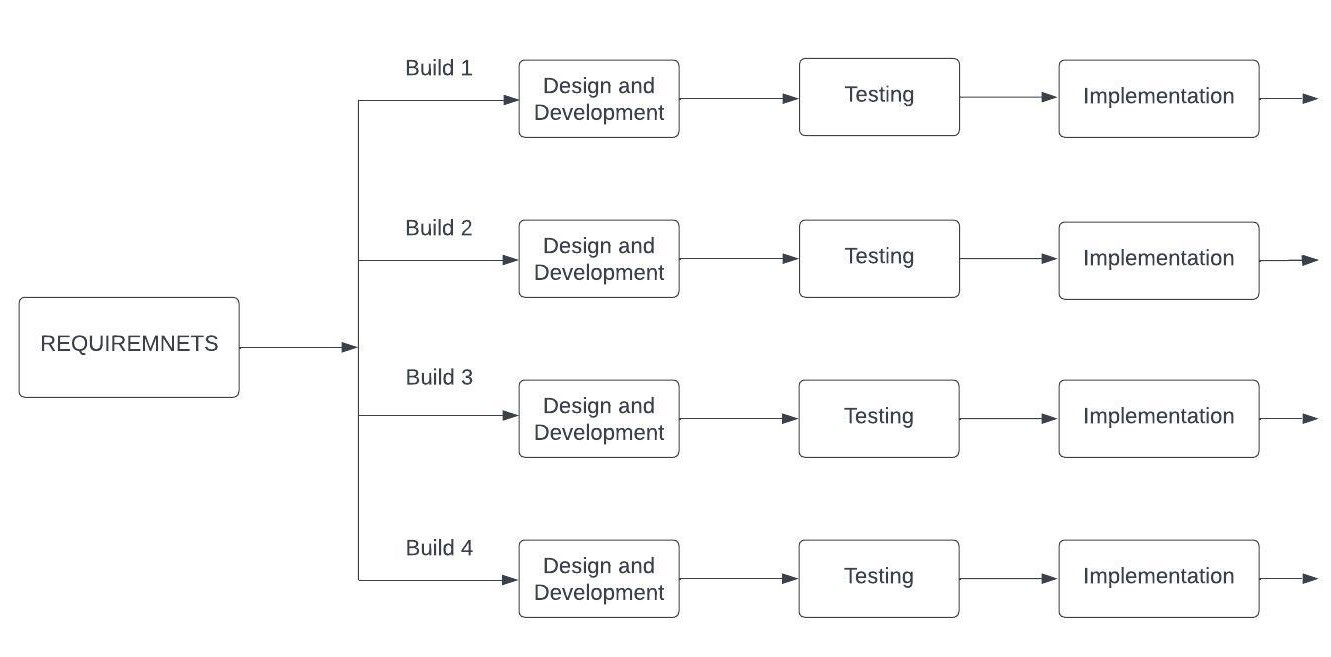
\includegraphics[width=5in]{images/sdlc1.jpg} 
	\caption{Incremental Model} %figure name
	\label{Incremental Model} % for referencing
\end{center}
\end{figure}

\chapter{Epilogue}
\vspace{-18pt}
%\section{Expected Output}
%\vspace{-18pt}
%Upon the completion of the project, the system will be able to take %input from the user and determine whether there is a tumor in the given input. 

\section{Work Completed}
\vspace{-18pt}

In our recent work, we have incorporated four well-known pre-trained models: Xception, InceptionV3, VGG-19, and ResNetV50 and compared their accuracies to gain insights into their respective strengths and weaknesses. Additionally, we implemented a custom AlexNet variant and evaluated its performance in comparison to the pre-trained models.

%
\includegraphics[width = in]{images/logo.png}
\begin{figure}[tbh] % tbh means top, bottom or here (priority: left to right)
\begin{center}
	%
\includegraphics[width = 3in]{images/logo.png}
	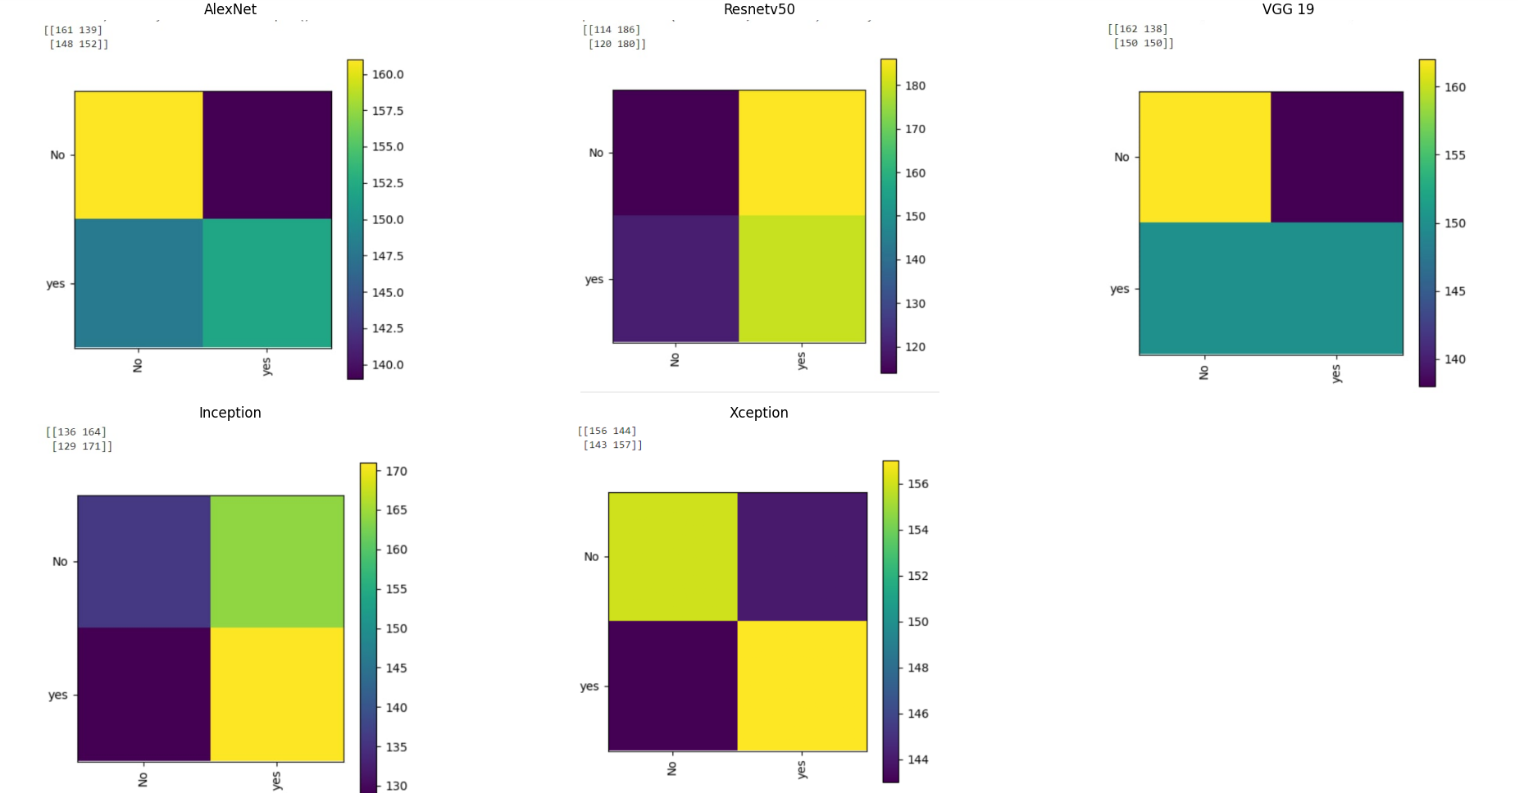
\includegraphics[width=5in]{images/confusion_matrix.png} 
	\caption{Comparision of confusion matrix} %figure name

	%\caption[Comparision of confusion matrix]{ \Comparision of confusion matrix
	\label{Comparision of confusion matrix}} % for referencing
\end{center}
\end{figure}
\begin{figure}[H] % tbh means top, bottom or here (priority: left to right)
\begin{center}
	%
\includegraphics[width = 3in]{images/logo.png}
	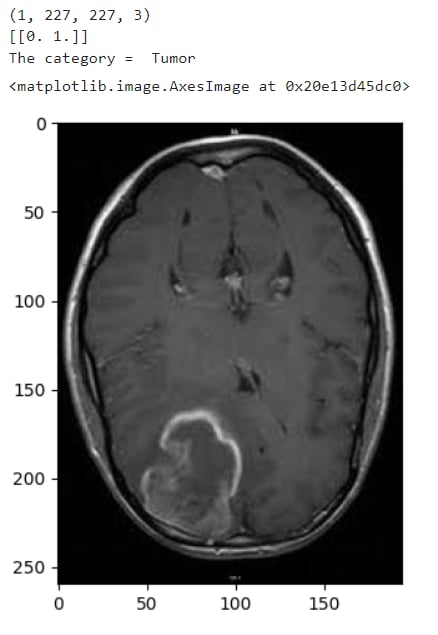
\includegraphics[width=3in]{images/tumor_image.jpg} 
	\caption{Output Image} %figure name
	\label{Output Image} % for referencing
\end{center}
\end{figure}

\begin{figure}[H] % tbh means top, bottom or here (priority: left to right)
\begin{center}
	%
\includegraphics[width = 3in]{images/logo.png}
	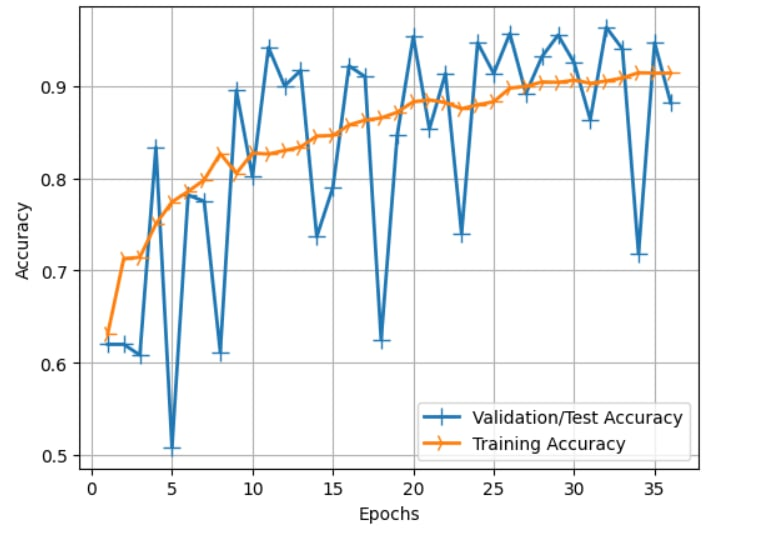
\includegraphics[width=3in]{images/accuracy.jpg} 
	\caption{Testing and Training Accuracy} %figure name
	\label{Testing and Training Accuracy} % for referencing
\end{center}
\end{figure}

\begin{figure}[H] % tbh means top, bottom or here (priority: left to right)
\begin{center}
	%
\includegraphics[width = 3in]{images/logo.png}
	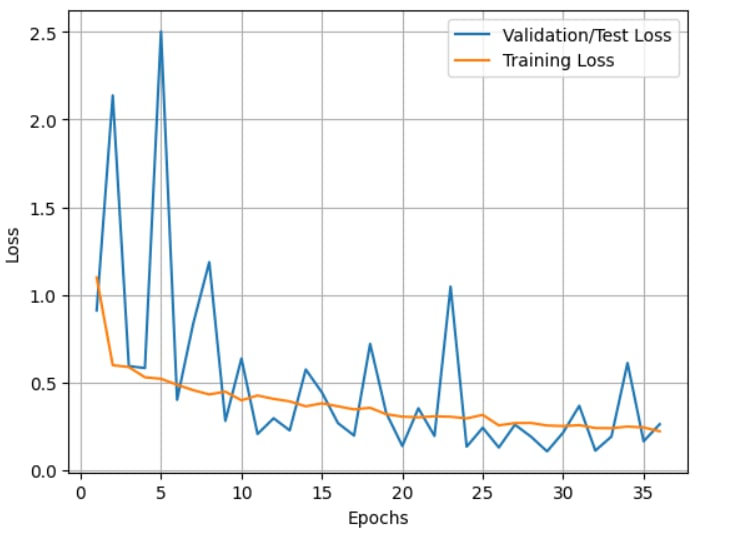
\includegraphics[width=3in]{images/loss.jpg} 
	\caption{Testing and Training Loss} %figure name
	\label{Testing and Training Loss} % for referencing
\end{center}
\end{figure}

\begin{figure}[H] % tbh means top, bottom or here (priority: left to right)
\begin{center}
	%
\includegraphics[width = 3in]{images/logo.png}
	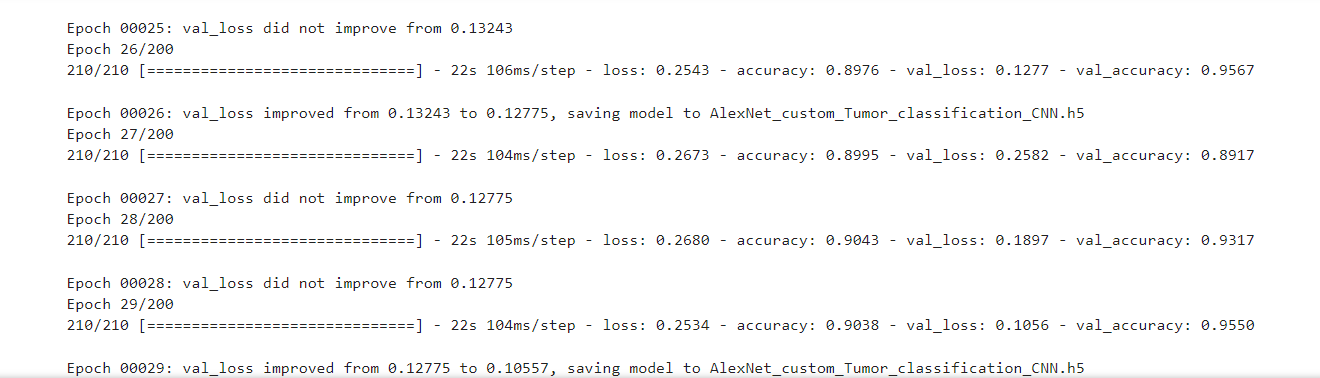
\includegraphics[width=3in]{images/epochs.png} 
	\caption{Epochs with Early Stopping} %figure name
	\label{Epochs with Early Stopping} % for referencing
\end{center}
\end{figure}
	


\section{Work Remaining}
\vspace{-18pt}
\begin{itemize}
\item Integrating SVM with the model
\item Creating UI for the model
\item Tuning the hyperparameters
\end{itemize}
%\chapter*{References}
%Reference
\renewcommand\bibname{REFERENCES} % Change heading to References
\bibliographystyle{IEEEtran} % to use IEEE Format for referencing
\addcontentsline{toc}{chapter}{References} % to add references in TOC
\bibliography{library} % specify the .bib file containing reference information 
\end{document}
